\section{\Acrfull{bsj} detection}

For detection of \glspl{bsj}, I used the five tools already introduced in
\cref{subsec:circrna_detection}.
As shown in \cref{fig:detection_bars}, find\_circ, CIRI2, DCC, and
circexplorer2 detect a similar number of \glspl{bsj}, while segemehl detects
almost ten times as many \glspl{bsj} as its closest competitor, DCC.

\begin{figure}[H] \centering

    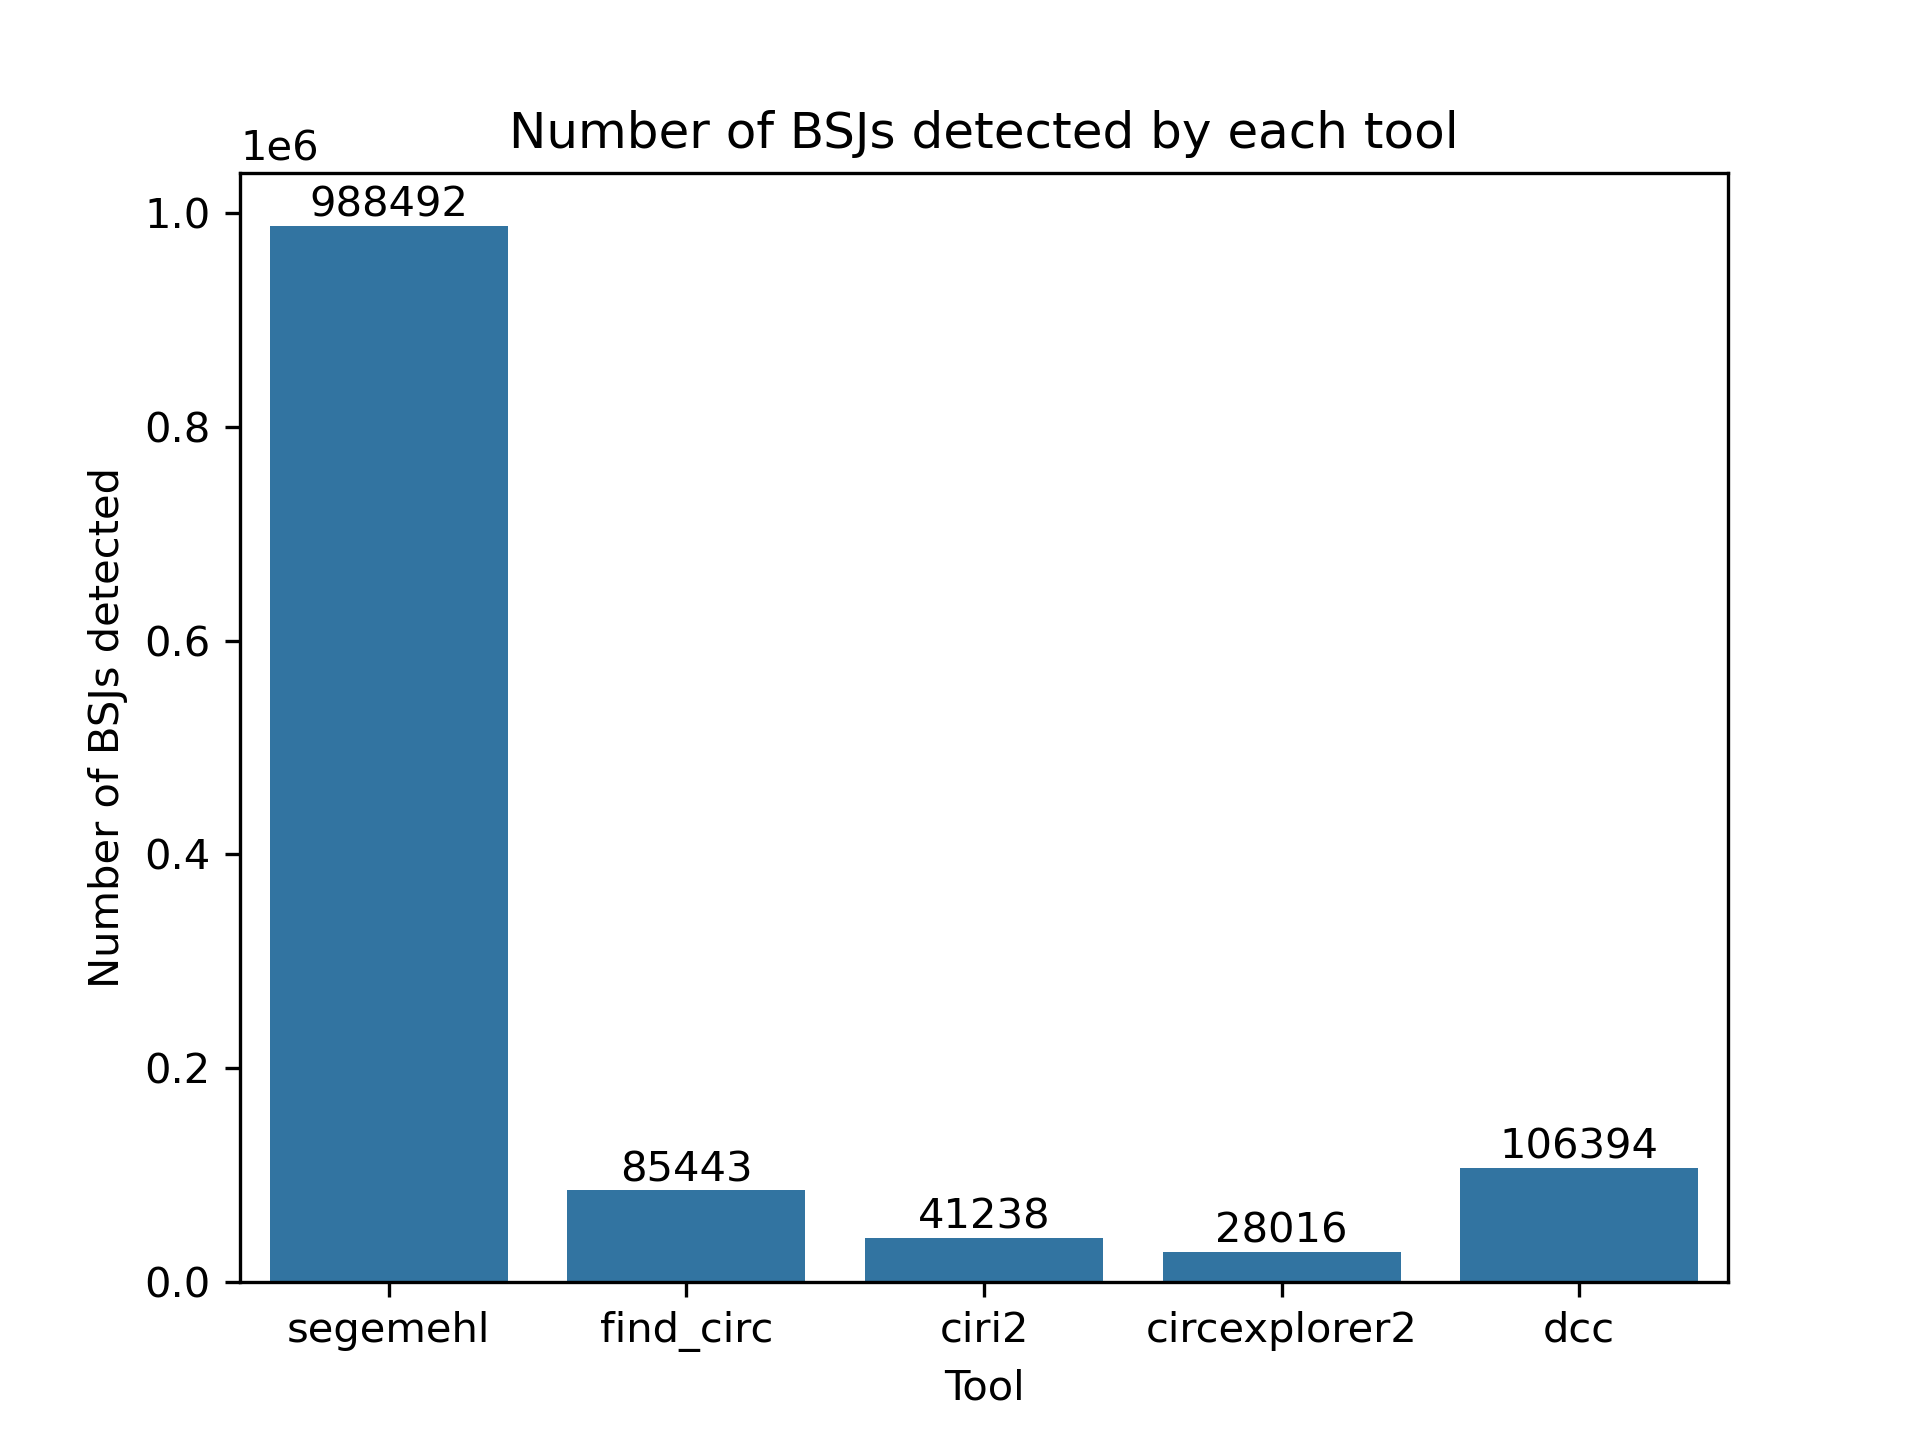
\includegraphics[width=0.6\textwidth]{chapters/4_results_and_discussion/figures/detection/n_bsjs_detected.png}
    \caption{Number of \glspl{bsj} detected by each tool.
        While find\_circ, CIRI2, DCC and circexplorer2 detect a similar number of
        \glspl{bsj}, segemehl detects a much larger number of \glspl{bsj}.
    }
    \label{fig:detection_bars}
\end{figure}
Similar behavior was previously observed by \textcite{zeng_comprehensive_2017},
where segemehl was among the top performers in terms of sensitivity, but also
had a high false positive rate.
The lowest numbers of \glspl{bsj} were detected by circexplorer2 and CIRI2,
which both have built-in filters to reduce false
positives\supercite{zhang_diverse_2016,gao_circular_2018}.

\subsection{Agreement between tools}

Although tools like CIRI2 and CircExplorer2 have shown good performance in
benchmarks, having multiple tools agree on the same \gls{bsj} can be a good
indicator of the reliability of the detection.

To assess the agreement between the tools, I used UpSet plots, which show the
overlap of \glspl{bsj} detected by different tools.
When identifying the overlap between tools, the most strict approach is to
consider only \glspl{bsj} with identical start and end positions and on the
same strand as the same \gls{bsj}.
The according plot is shown in \cref{fig:detection_upset_0}.
While there are a total of x \glspl{bsj} detected by at least two tools, only y
\glspl{bsj} are detected by three tools, and none are detected by four or five
tools.

\begin{figure}[H]
    \centering

    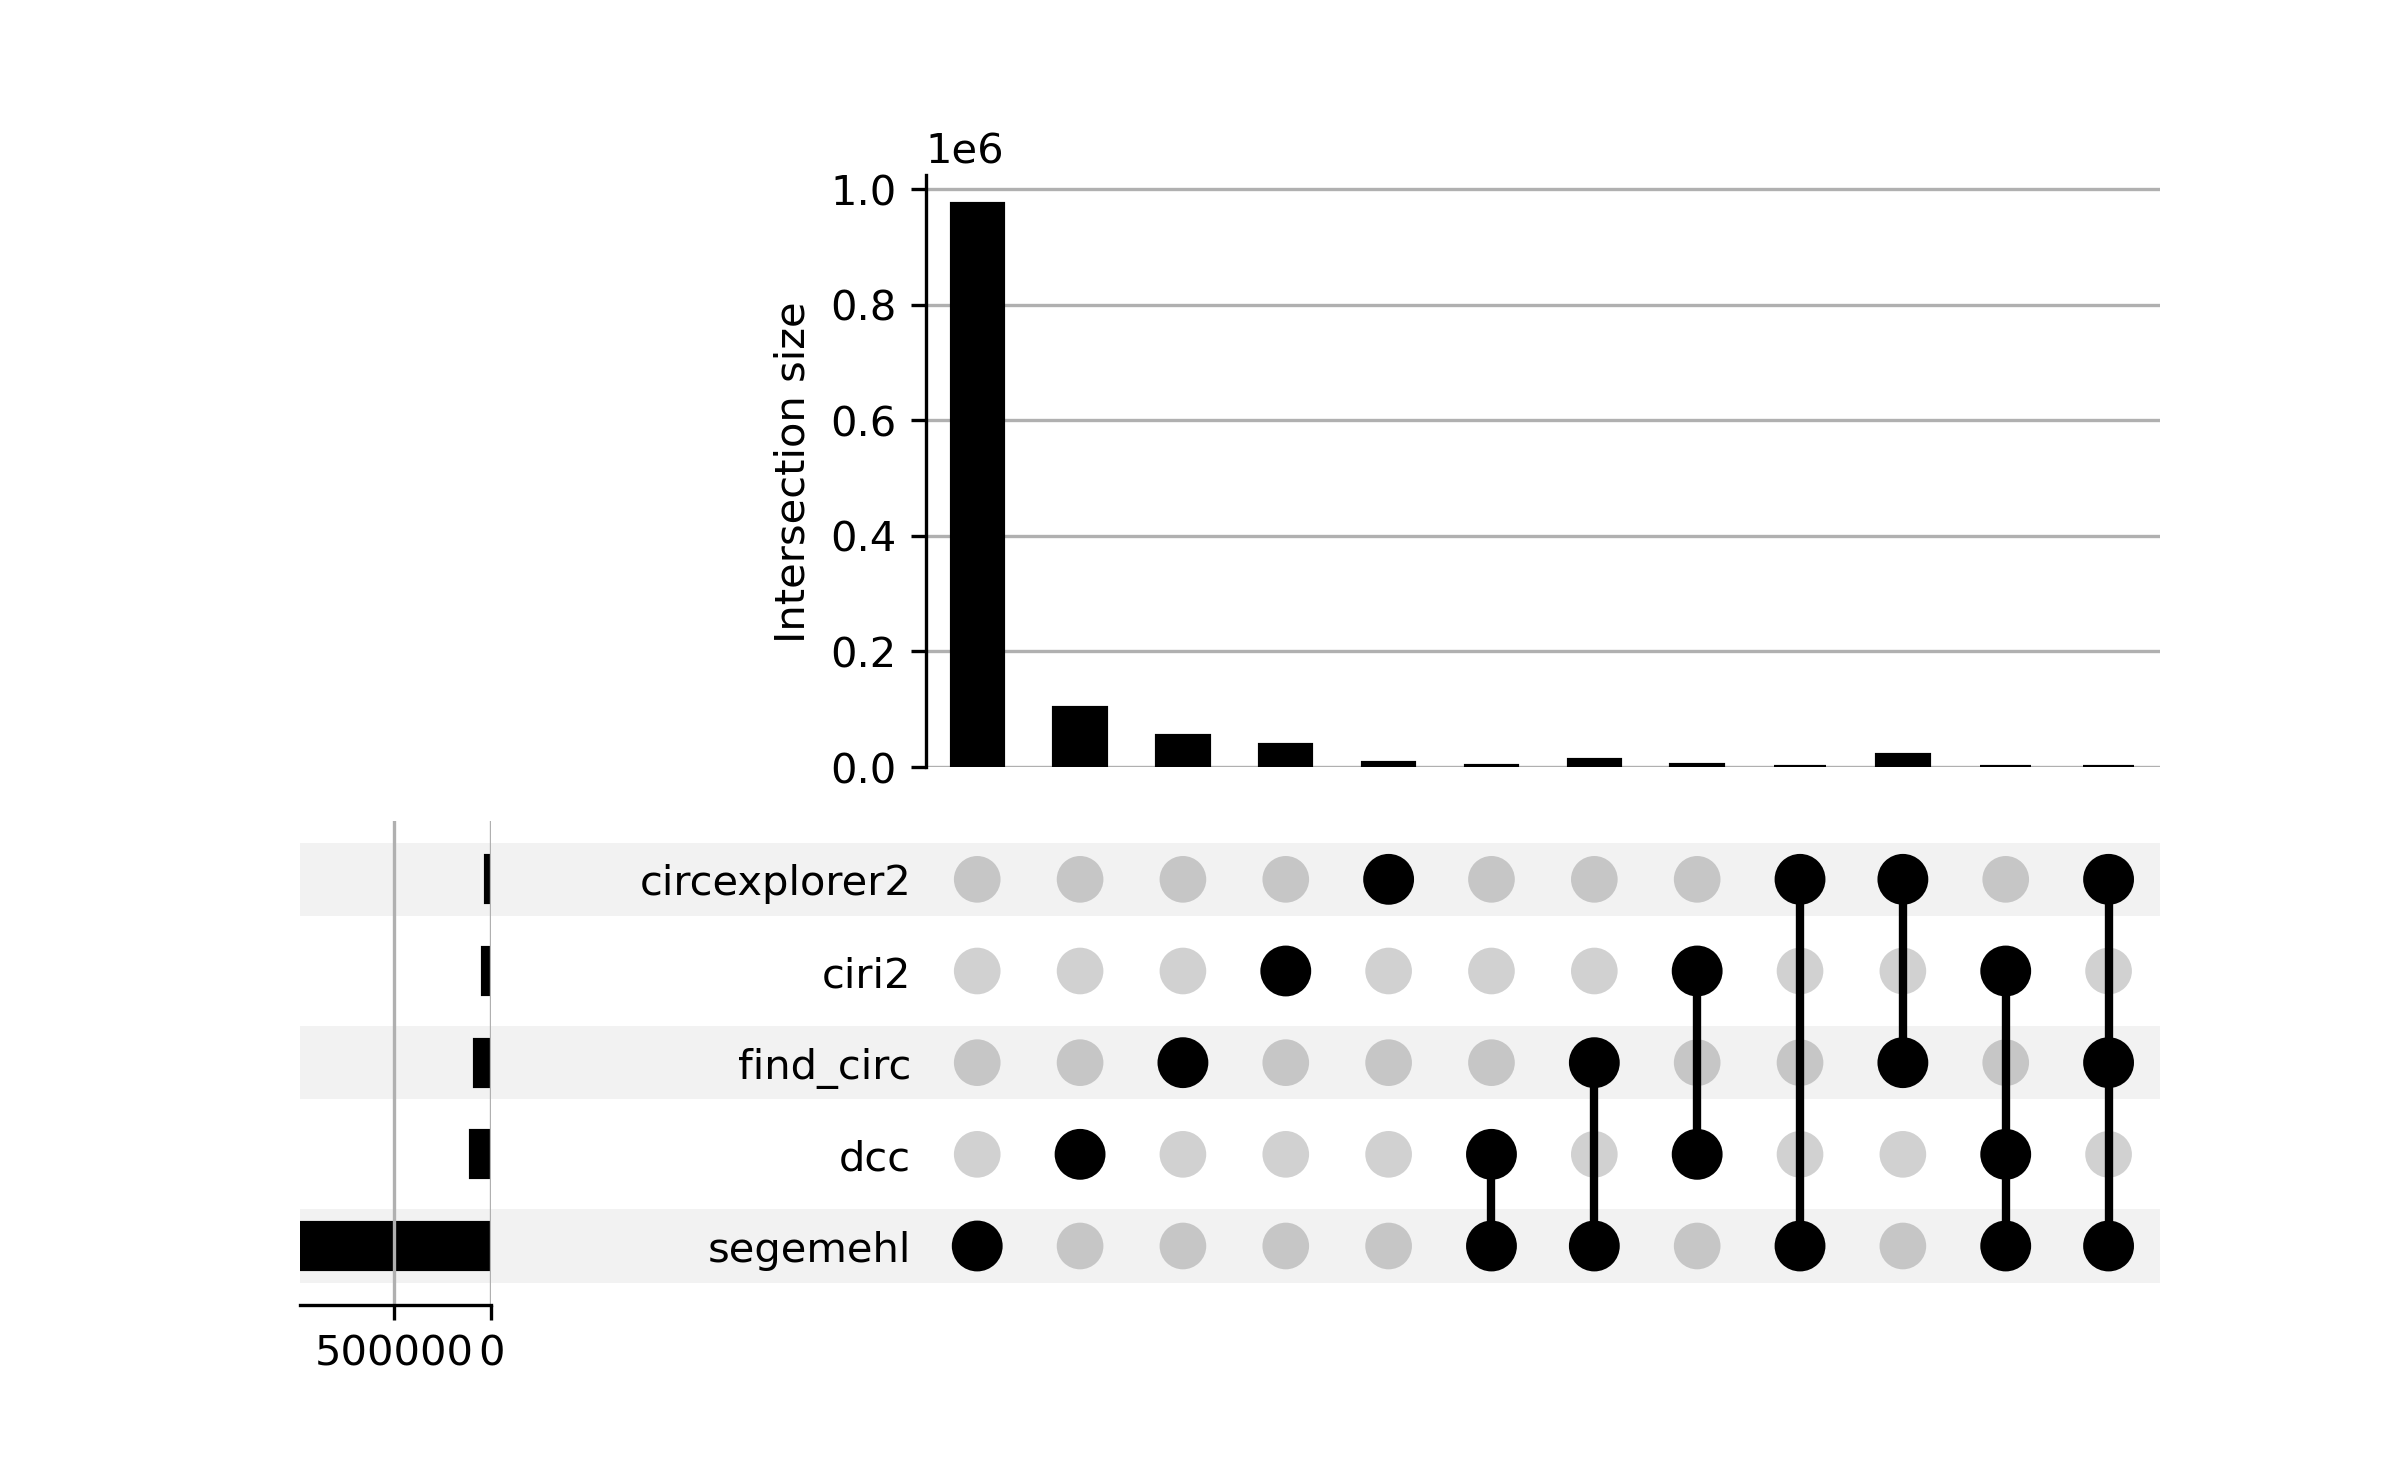
\includegraphics[width=\textwidth]{chapters/4_results_and_discussion/figures/detection/upset/shift_0_stranded.png}
    \caption{Upset plot illustrating the overlap between \glspl{bsj} detected
        by
        different tools.
        Only \glspl{bsj} with identical start and end positions are considered the
        same.
        Only combinations with at least 10 common \glspl{bsj} are shown.
        While most detection tools show similar results, segemehl stands out with the
        largest number of \glspl{bsj} detected by only one tool.
        On the other hand, it is also involved in most of the combinations with 2-3
        tools.
    } \label{fig:detection_upset_0} \end{figure}

As this agreement is relatively low, I investigated the detected \glspl{bsj}
more closely and found that tools often have very similar \glspl{bsj}, but on
different strands and with slight differences in the start and end positions.

\subsubsection{The role of the \textit{max shift} parameter}
In order to quantify how frequently the slight mismatches occur, I introduced a
\textit{max shift} parameter.
With this parameter, if tool A detects a \gls{bsj} and tool B detects another
\gls{bsj}, where the start and end positions differ by at most \textit{max
    shift} nucleotides, both \glspl{bsj} are considered to be supported by both
tools.
A more detailed explanation is given in \cref{fig:detection_shift_schematic}.

\begin{figure}[H] \centering

    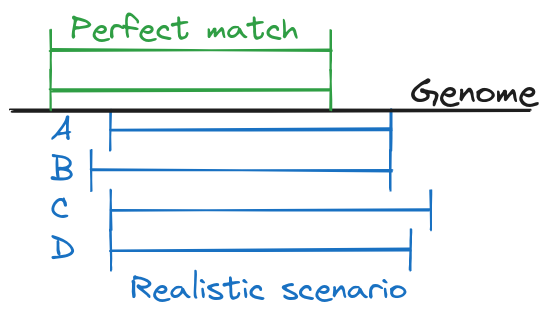
\includegraphics[width=0.7\textwidth]{chapters/4_results_and_discussion/figures/grouping.png}
    \caption{Schematic illustrating two different scenarios of \gls{bsj}
        matches
        across tools.
        In the green scenario, the \glspl{bsj} are exactly the same.
        This is what is required in order to be counted as a match in
        \cref{fig:detection_upset_0}.
        However, this rarely occurs in practice.
        More frequently, the scenario illustrated in blue occurs.
        Here, tools detect very similar \glspl{bsj}, with only a few nucleotides
        difference.
        In order to account for this, a \textit{max shift} parameter is introduced.
        While in the blue scenario, all \glspl{bsj} would only be supported by one
        tool, with a \textit{max shift} of 1, the result would change drastically.
        The \gls{bsj} marked as A would be supported by two others (B and D), similarly
        B would be supported by two others (A and D).
        C would only be supported by D, as both the ends of both A and B differ by more
        than 1.
        D would be supported by all others.
    }
    \label{fig:detection_shift_schematic}
\end{figure}

In order to quantify the magnitude of the effect of the \textit{max shift}
parameter, I calculated the level of agreement between tools for different
values of \textit{max shift}.
The results are shown in \cref{fig:shift_agreement}.

\begin{figure}[H]
    \centering

    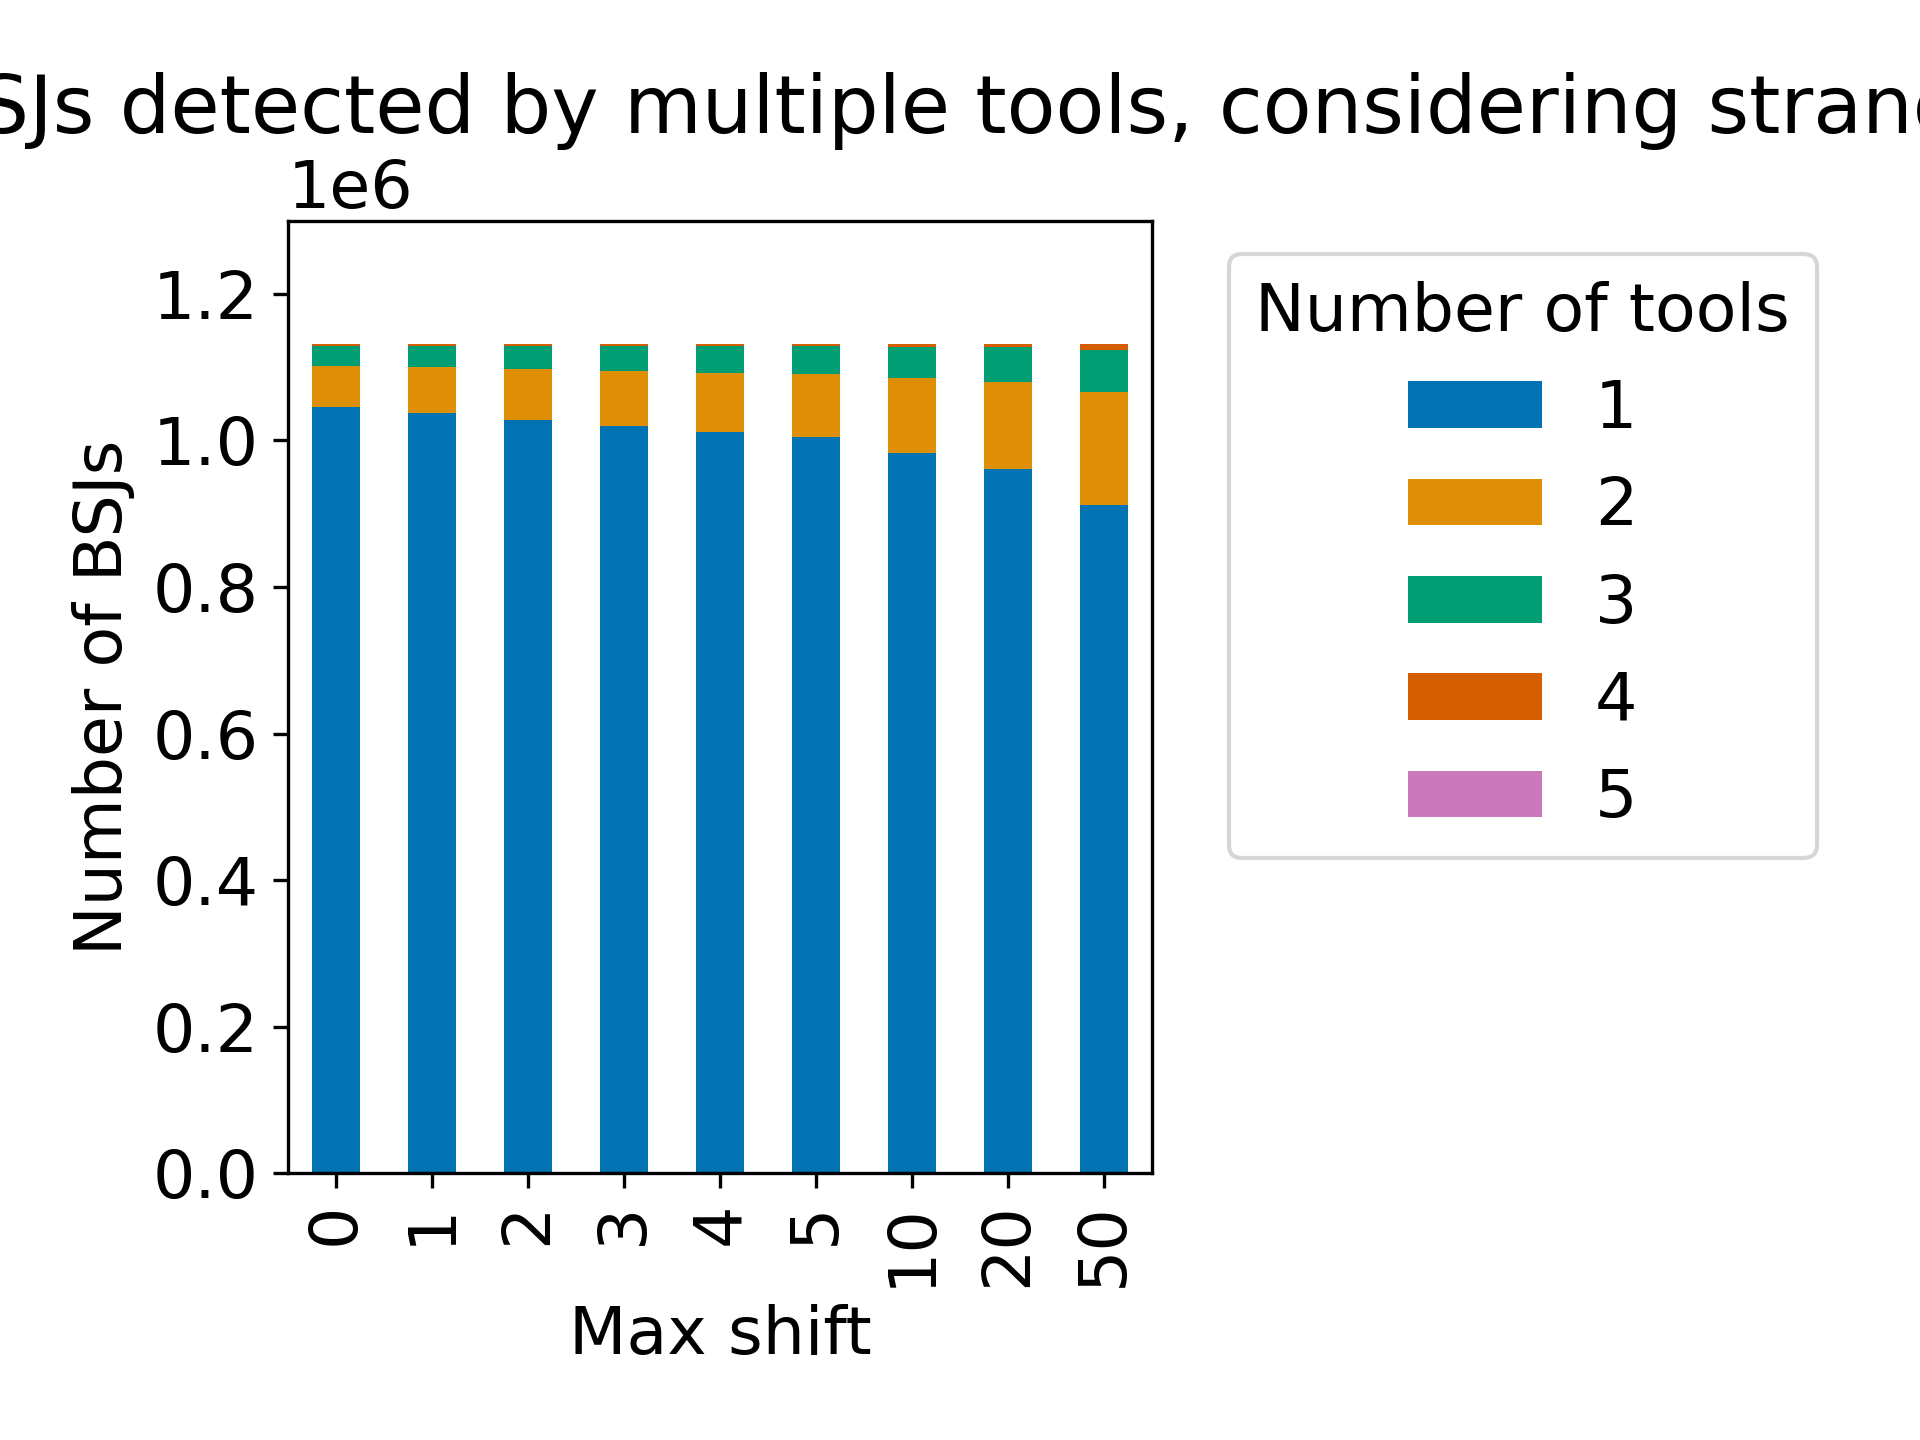
\includegraphics[width=0.7\textwidth]{chapters/4_results_and_discussion/figures/detection/shift_agreement_stranded.png}
    \caption{Stacked bar plot showing the level of agreement between tools for
        different values of the \textit{max shift} parameter.
        While the distribution changes drastically when increasing the \textit{max
            shift} parameter from 0 to 1, the distribution remains relatively stable for
        higher values.
        While the number of \glspl{bsj} detected by 2-3 tools continues to increase
        when raising the \textit{max shift} parameter to 20 or 50, the number of
        \glspl{bsj} detected by 4-5 tools remains nearly constant.
    }
    \label{fig:shift_agreement_stranded}
\end{figure}

As shown in \cref{fig:shift_agreement_stranded}, the distribution of the number
of tools supporting a \gls{bsj} changes drastically when increasing the
\textit{max shift} parameter from 0 to 1.
However, the distribution remains relatively stable, especially for agreement
between four or five tools.
Increasing the \textit{max shift} parameter to large values does have an effect
on the number of \glspl{bsj} detected by two or three tools, but this comes
with the risk of increasing the number of false positives, since this way
\glspl{bsj} with a relatively large difference in start and end positions are
still considered as evidence for each other.

\subsubsection{The role of strandedness}

\begin{figure}[H]
    \centering

    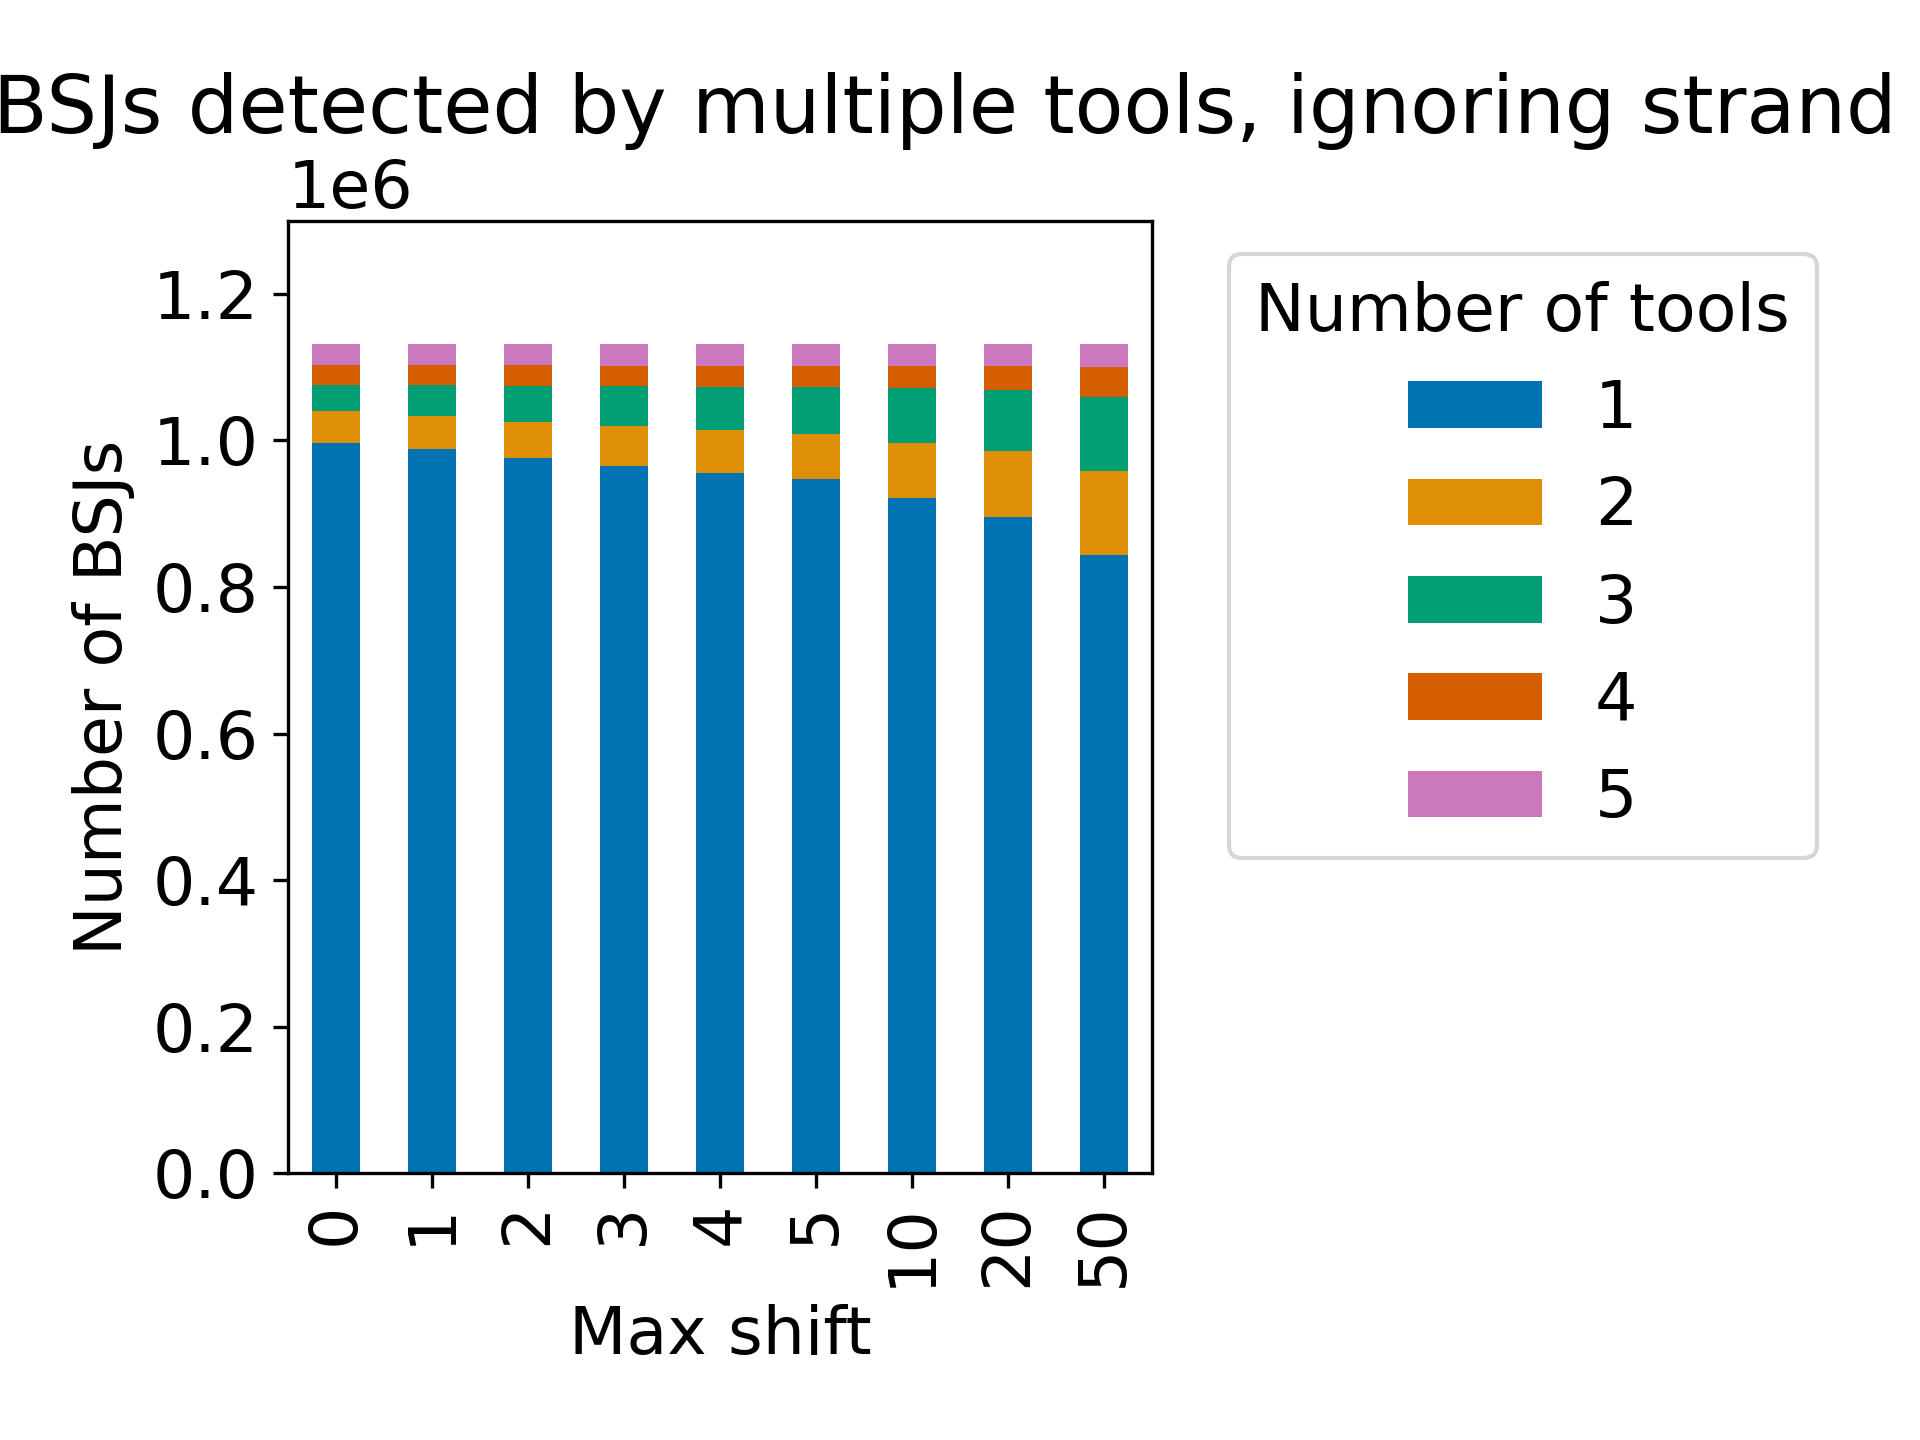
\includegraphics[width=0.7\textwidth]{chapters/4_results_and_discussion/figures/detection/shift_agreement_unstranded.png}
    \caption{Stacked bar plot showing the level of agreement between tools for
        different values of the \textit{max shift} parameter.
        While the distribution changes drastically when increasing the \textit{max
            shift} parameter from 0 to 1, the distribution remains relatively stable for
        higher values.
        While the number of \glspl{bsj} detected by 2-3 tools continues to increase
        when raising the \textit{max shift} parameter to 20 or 50, the number of
        \glspl{bsj} detected by 4-5 tools remains nearly constant.
    }
    \label{fig:shift_agreement_unstranded}
\end{figure}

\subsubsection{Selecting thresholds}

For the following analyses, I chose a \textit{max shift} parameter of 3 and a
minimum agreement of 4 tools, as this appeared to be a good compromise between
sensitivity and specificity.
The resulting UpSet plot is shown in \cref{fig:detection_upset_3}.

\begin{figure}[H]
    \centering

    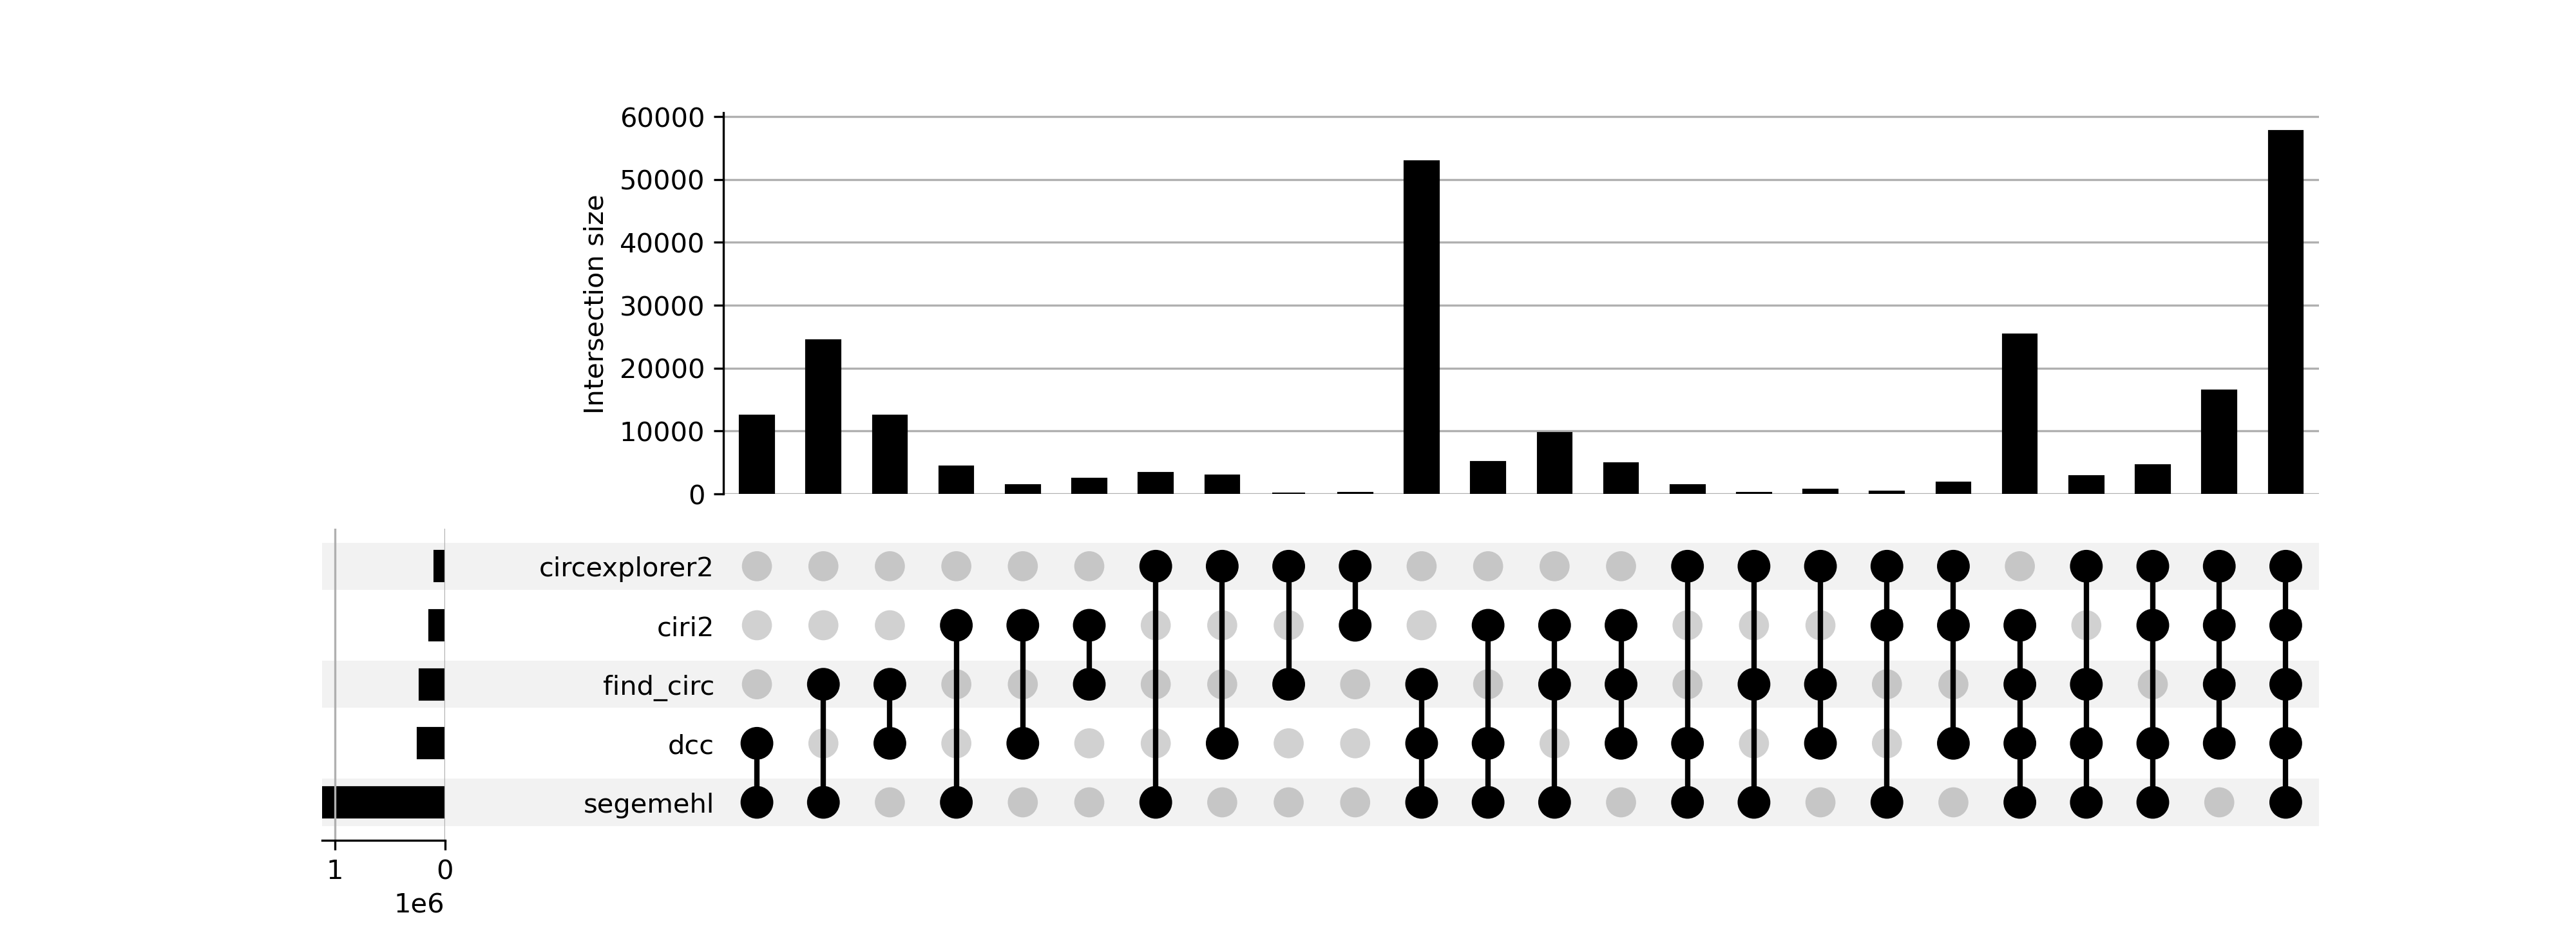
\includegraphics[width=\textwidth]{chapters/4_results_and_discussion/figures/detection/upset/shift_3_unstranded.png}
    \caption{Upset plot illustrating the overlap between \glspl{bsj} detected
        by
        different tools.
        Agreement was calculated using a \textit{max shift} of 3.
        Only combinations including at least 2 tools and 10 common \glspl{bsj} are
        shown.
    }
    \label{fig:detection_upset_3}
\end{figure}

\subsection{circRNA types}

\begin{figure}[H]
    \centering

    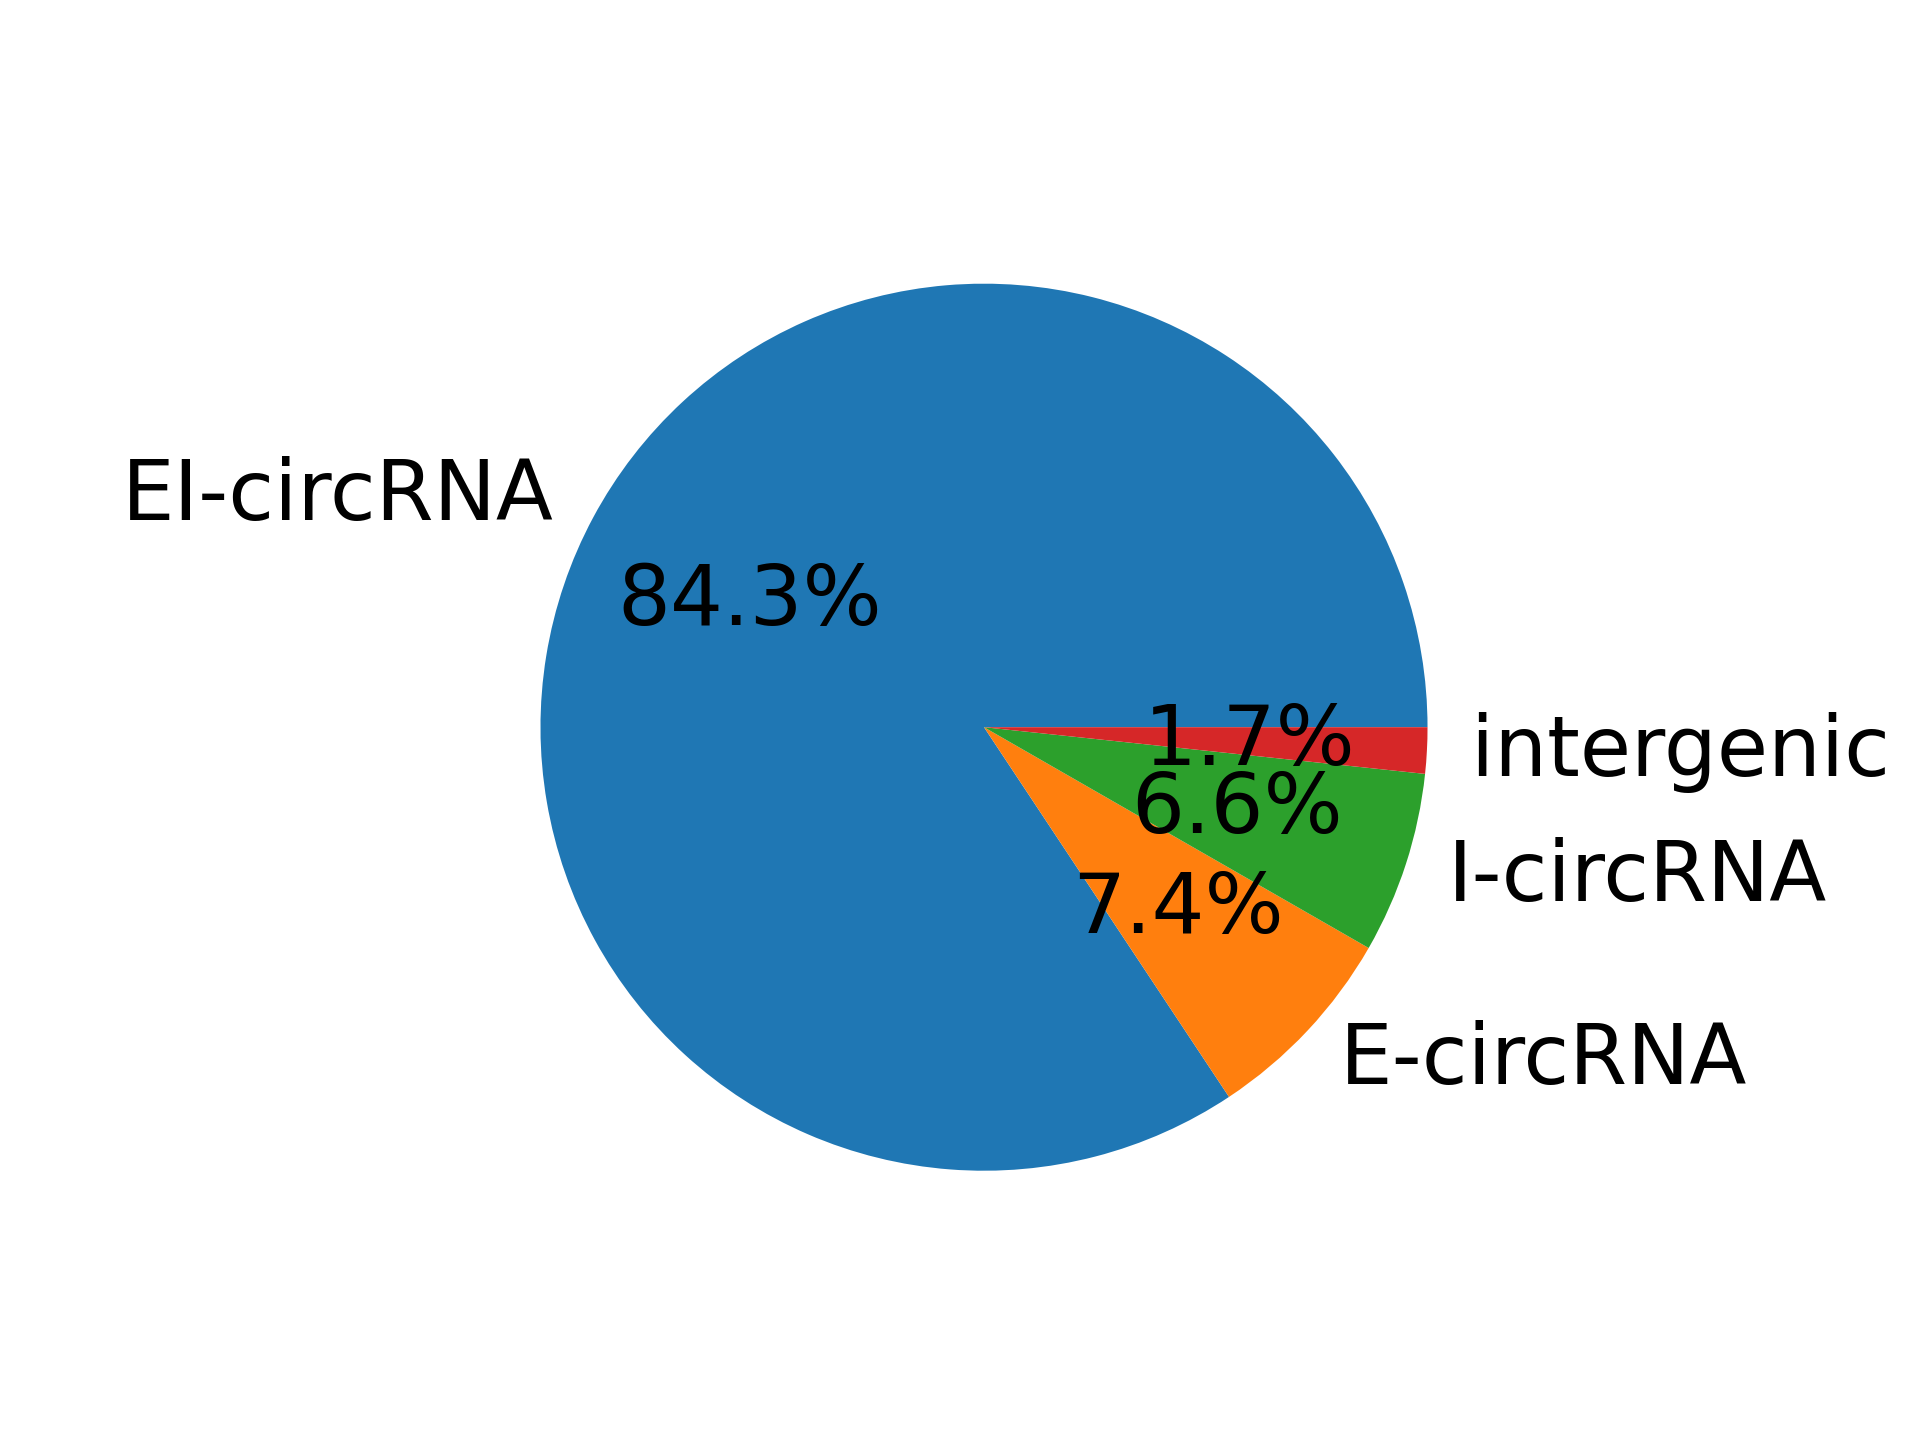
\includegraphics[width=0.5\textwidth]{chapters/4_results_and_discussion/figures/detection/types.png}
    \caption{Pie chart showing the distribution of different types of
        \glspl{crna} detected by the pipeline.
        While according to literature \glspl{e-crna} are the most abundant type of
        \glspl{crna}, here we see \glspl{ei-crna} as the most abundant type.
        This is most likely due to the fact that we only know the start and end
        positions of the \glspl{bsj}, but not the internal structure of the
        \glspl{crna}.
        Thus, \glspl{crna} are only labeled as \glspl{e-crna} if they are fully
        contained in a single exon.
        If they span multiple exons (thus, overlapping with at least one intron), they
        are labeled as \glspl{ei-crna}.
    }
    \label{fig:circrna_types}
\end{figure}

\subsection{Database agreement}
\begin{figure}[ht] \begin{tabular}{cc}
        \begin{subfigure}{0.5\textwidth} \centering

            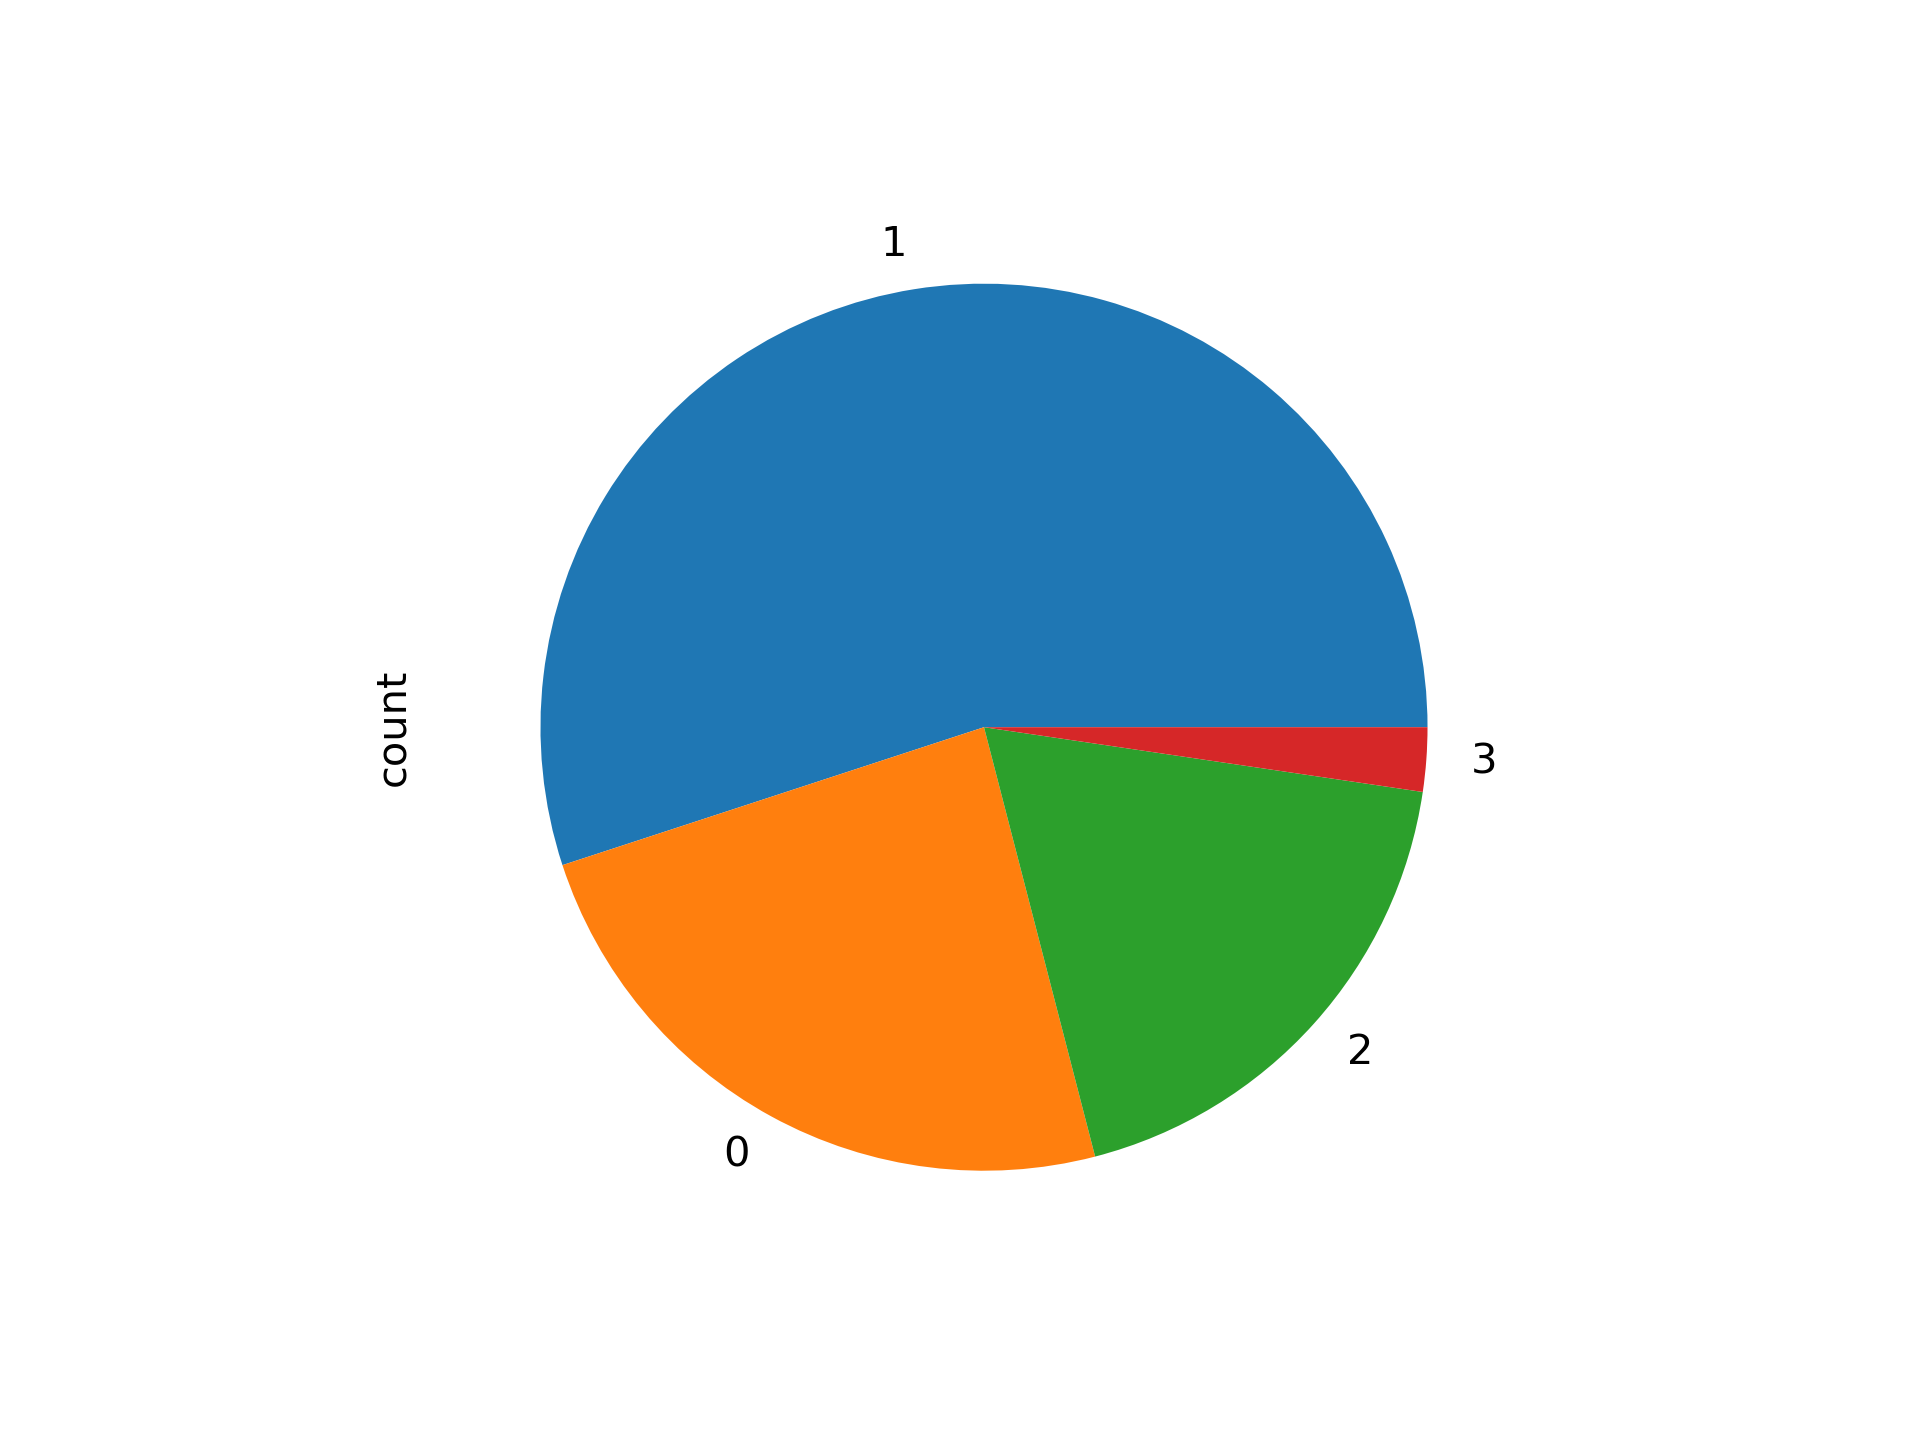
\includegraphics[width=\linewidth]{chapters/4_results_and_discussion/figures/detection/database_count.png}
            \caption{Fractions of \glspl{crna} supported by
                different numbers of databases}
            \label{fig:db_pie}
        \end{subfigure}
        \begin{subfigure}{0.5\textwidth}
            \centering

            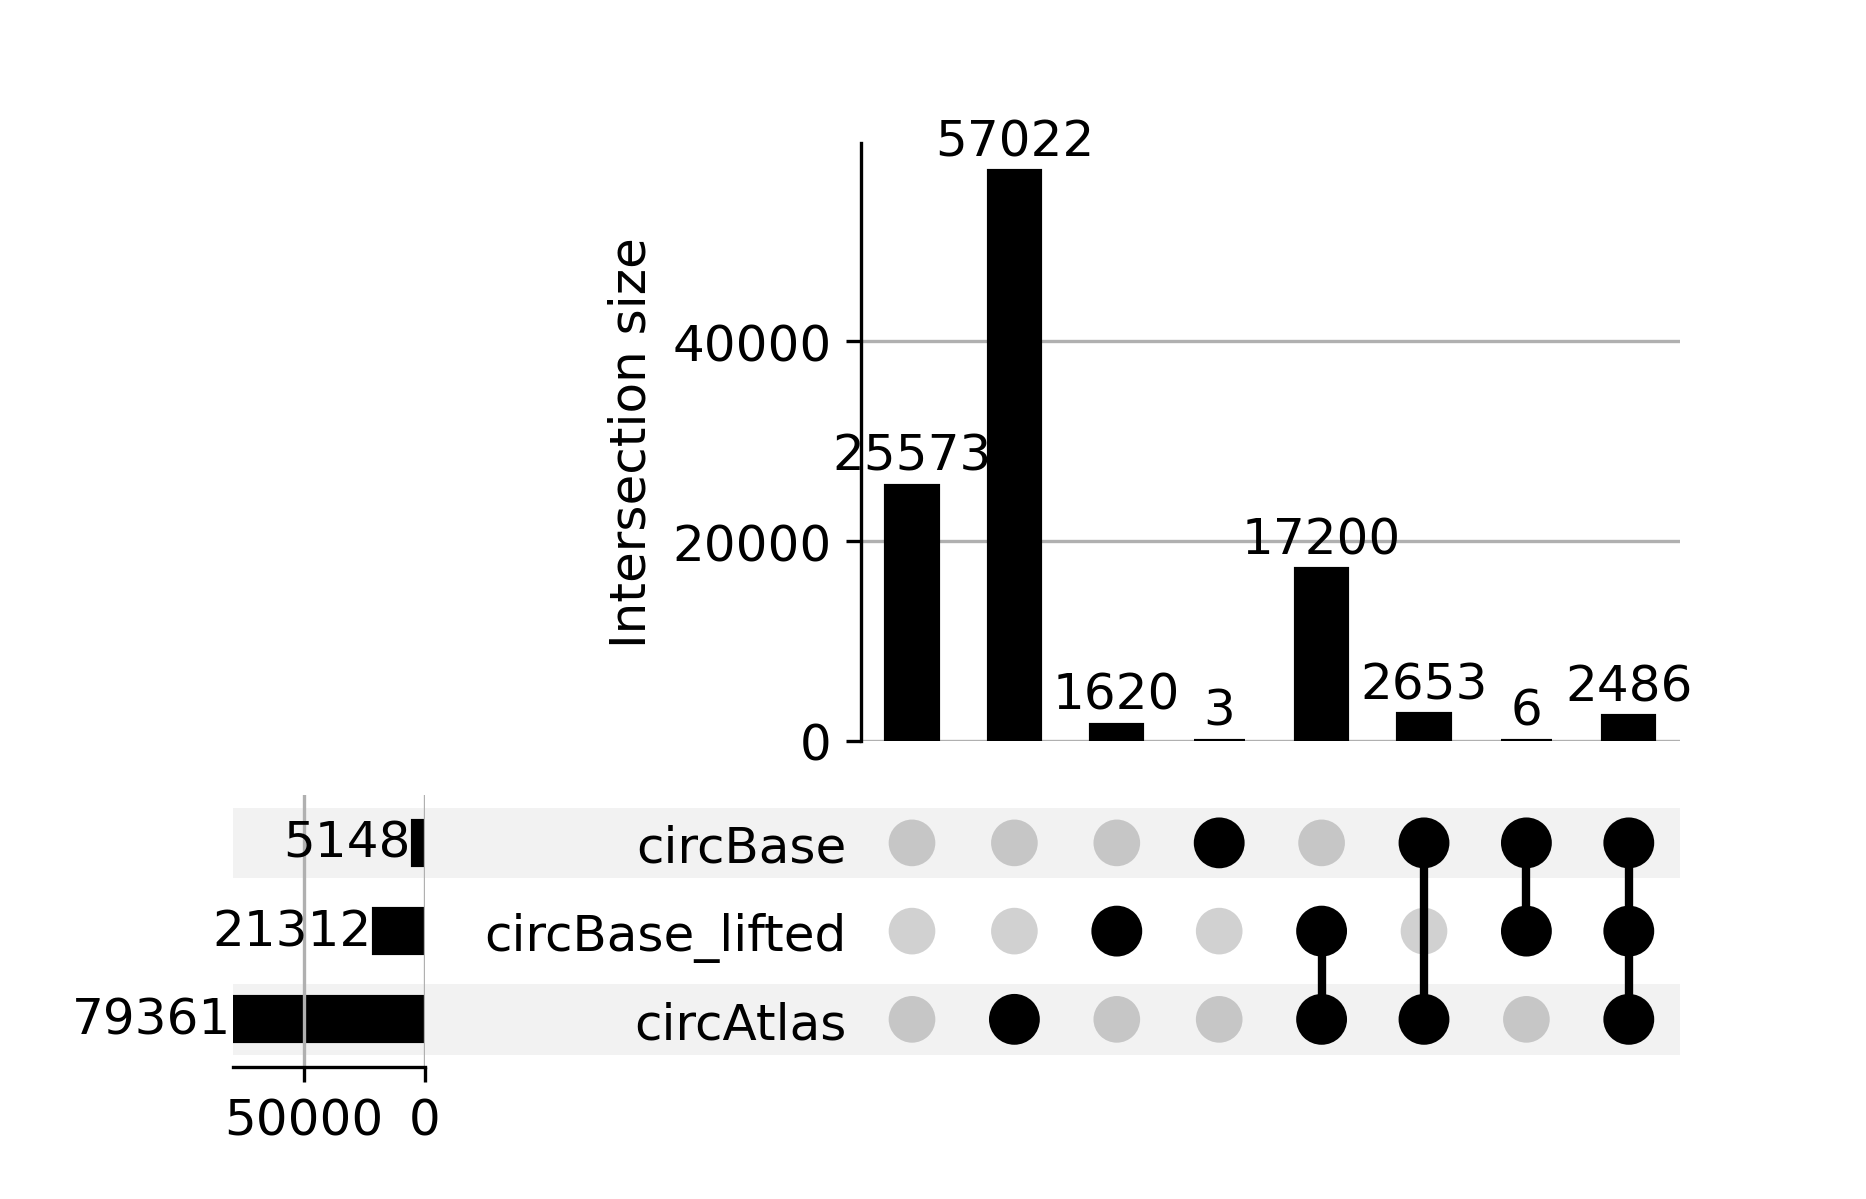
\includegraphics[width=\linewidth]{chapters/4_results_and_discussion/figures/detection/database_upset.png}
            \caption{Agreement between detected
                \glspl{bsj} and databases}
            \label{fig:db_upset}
        \end{subfigure} &

    \end{tabular}
    \caption{As \cref{fig:db_pie} shows, while there is a large fraction of
        \glspl{crna} without any
        database match, more than 50\% of detected \glspl{crna} at least one
        hit.
        As shown in \cref{fig:db_upset}, most hits are from circAtlas, which is most
        likely due to the fact that it is the largest database.
        While both circBase and circBase\_lifted have some exclusive hits, the majority
        of their hits are shared with circAtlas.
    }
    \label{fig:db_agreement}
\end{figure}
